\chapter{Contexte théorique et expérimental}
    \chapterprecishere{
        ``Potentielle citation sans aucun rapport avec le sujet"\par\raggedleft--- \textup{Personne inconnue}, contexte à déterminer
    }
    
    Le but de ce chapitre est de couvrir en quelques pages l'histoire des neutrinos, d'un point de vue théorique comme expérimental, de leur découverte jusqu'aux questions encore non résolues.
    
    \section{De la nécessité théorique à la découverte du neutrino}
    
        \subsection{Le spectre de désintégration \texorpdfstring{$\beta$}{b} : besoin d'une nouvelle particule}
    
        \subsection{Premières observations directes du neutrino}
    
        \subsection{Les 3 familles de neutrinos}
        
        \subsection{Dirac vs Majorana}\label{sec::dirac_majorana}
    
    \section{Le paradigme des oscillations des neutrinos}
    
        \subsection{Genèse de la théorie}
        
            On désigne habituellement un neutrino par sa saveur : neutrinos muonique($\nu_{\mu}$), électronique($\nu_e$) ou tauique$\nu_{\tau}$. Un neutrinos est dans l'un de ces 3 "états de saveur" si il est produit par le lepton qui y correspond, ou si il produit ce lepton en interagissant avec son environnement. Rien, à priori, n'oblige le lepton qui créé le neutrino à être de même saveur que le lepton créé par le neutrino après interaction. Le premier à avoir soulevé ceci est Bruno Pontecorvo, même si il ne l'a pas fait en ces termes. En effet, au moment de la publication de ses deux premiers articles\cite{Pontecorvo:1957cp,Pontecorvo:1957qd} sur le sujet à la fin des années 60, il n'était pas connu qu'il y avait plusieurs saveurs de neutrino. B.~Pontecorvo parlait de possible transition entre neutrino et antineutrino du fait que le neutrino soit neutre, inspiré par les travaux de Gell-Mann et Païs\cite{Gell-Mann1955} sur la conversion du $\overline{K^0}$ en  $K^0$. Dans son article suivant en 1968\cite{Pontecorvo1968}, tout en gardant la possibilité de conversion des neutrinos vers les antineutrinos, il introduit la possibilité d'une conversion du neutrino électronique vers le neutrino muonique, découvert en 1962\cite{Danby1962}. Il prédira également deux résultats importants :
            \begin{itemize}
                \item Si les masses des neutrinos ne sont pas nulles et que la charge leptonique n'est pas être conservée, les neutrinos peuvent changer de saveur
                \item Un déficit de neutrinos en provenance du soleil d'un facteur 2 environ par rapport au prédiction du modèle solaire standard est attendu dans ce cas
            \end{itemize}
            La première prédiction implique de la physique au delà du modèle standard de la physique des particules, puisque ce dernier suppose que les masses des neutrinos sont nulles. Mais ceci n'est pas imposé par la théorie : il a été expérimentalement observé dans toutes les expériences à ce jour que les neutrinos se comportent, si ce n'est comme des particules de masses nulles, comme des particules de masse suffisamment faible pour être négligée. 
            La seconde prédiction fut vérifiée en 1970 par la Brookhaven Solar Neutrino Experiment\cite{Bahcall1976}, qui trouva un déficit compris entre 2 et 3. Il ne s'agissait alors pas encore d'une preuve, d'autre théorie pouvant expliquer ce phénomène, mais c'était un indice qui a incité les chercheurs à creuser la question.
            
            Le changement de saveur $\nu_e\rightleftharpoons\nu_{\mu}$ avait été envisagé également entre 1962 et 1963 par deux groupes de physiciens, Katayama, Matumoto, Tanaka et Yamada\cite{Nakagawa1963} puis que Ziro Maki, Masami Nakagawa and Shoichi Sakata\cite{Maki1962}. Ces quatre derniers donneront leurs noms, avec Pontecorvo, à la célèbre matrice \gls{pmns} décrite plus loin. Leur point de départ était différent de celui de Pontecorvo, puisqu'ils visaient à créer une théorie unifiant les leptons et les hadrons. Ils sont également arrivé à la conclusion qu'une oscillation des neutrinos implique que ces derniers doivent avoir des masses non nulles.
            
            En 2015, Arthur~B.~McDonald et Takaaki Kajita ont reçu le prix Nobel de physique pour "pour la découverte des oscillations des neutrinos, qui montre que les neutrinos ont une masse". Les deux expériences ayant fait cette découverte sont SNO\cite{Aharmim2013} et Super-Kamiokande\cite{Fukuda1998}.
            
            \begin{figure}[htbp]
                \begin{subfigure}[t]{0.56\textwidth}
                    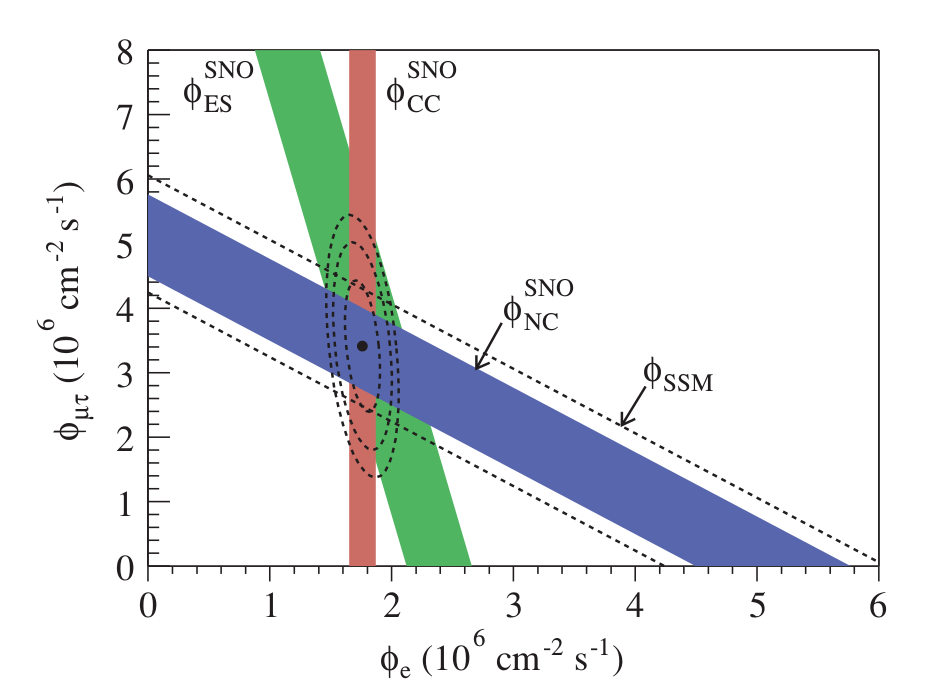
\includegraphics[width=\textwidth]{Chapitre_1/pictures/SNO_plot.png}
                    \caption{Mesure des composantes $\nu_{\mu}$ et $\nu_{\tau}$ du flux de neutrino solaire contre la composante $\nu_e$\cite{Aharmim2013}. Le flux total mesuré ($\phi_{NC}^{SNO}$) est consistant avec le flux total prédit ($\phi_{SSM}$). La composante électrinique du flux ($\phi_{CC}^{SNO}$), qui devrait constituer $100\%$ du flux sans oscillations, n'en représente que $35\%$, ce qui indique un changement de saveur.}
                    \label{fig::SNO_plot}
                \end{subfigure}
                \hfill 
                \begin{subfigure}[t]{0.4\textwidth}
                    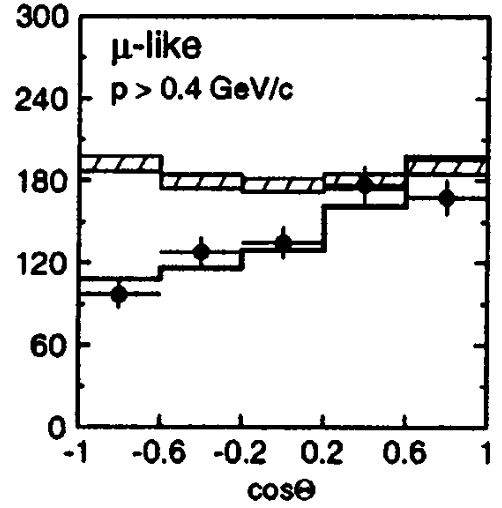
\includegraphics[width=\textwidth]{Chapitre_1/pictures/superK_plot.png}
                    \caption{Nombre de neutrinos muoniques mesurés par Super-Kamiokande (traits pleins) et prédit par le Monte Carlo (traits pointillés) pour un an et demi de prise de donnée contre l'angle zénithal avec lequel le neutrino arrivait\cite{Fukuda1998}. Un cosinus négative correspond à un neutrino ayant traversé la Terre. La différence entre observation et prédiction à grand angle indique une disparition des neutrinos muonique.}
                    \label{fig::superK_plot}
                \end{subfigure}
            \end{figure}
            
            SNO détectait les neutrinos solaires, par interaction par courant chargé (CC) et par courant neutre (CN), permettant d'avoir accès à la fois au flux de neutrinos électroniques (CN et CC) et au flux de neutrios muoniques et tauiques (CN). Comme le montre la \autoref{fig::SNO_plot}, la somme des trois flux correspond bien au flux total prédit par le modèle solaire standard alors que le flux de neutrinos électronique est inférieur aux prédiction, montrant qu'une partie du flux change de saveur mais que le flux total est conservé.
            
            Super-Kamiokande détectait des neutrinos issues des interactions de rayons cosmiques avec l'atmosphère. Il pouvait ainsi comparer les flux des neutrinos pour différents angles zénithaux, correspondant à des créations du neutrino allant de juste au dessus du détecteur (angle nul) à l'autre bout du globe (angle de $\pi$). Comme nous allons le montrer plus loin, la probabilité qu'a un neutrino de changer de saveur dépend de la distance parcoure (équation \eqref{eq::proba_oscillation}). Une dépendance du flux en l'angle zénithal a donc indiqué un phénomène de changement de saveur. La figure \autoref{fig::superK_plot} montre cette dépendance pour des événements de neutrinos muoniques.
    
        \subsection{Pourquoi "Oscillations"?}
            La base de la théorie de l'oscillation des neutrinos est de dire que les états $\nu_e$ $\nu_{\mu}$ et $\nu_{\tau}$ sont -- par définition -- des états propres du lagrangien d'interaction, mais pas forcément des états propres de l'hamiltonien, appelés également états propres de masse. Autrement dit, il n'est pas forcément possible de décrire la propagation dans l'espace temps d'un état de saveur. Partons du principe que les états de saveurs des neutrinos ne sont en effet \textit{pas} des états propres de masse et regardons les conséquences. 
            
            \subsubsection{Conventions de notation}
            \begin{itemize}
                \item $\hbar = c = 1$ (système d'unité naturelle)
                \item Nous supposerons que toutes les fonctions d'ondes décrites sont suffisamment loin de leur source pour être considérées comme des ondes planes. Les expériences de neutrinos vérifient généralement facilement cette conditions.
                \item $\nu_e$ $\nu_{\mu}$ et $\nu_{\tau}$ sont les états propres de saveur. Un neutrino est dans un de ces états au moment de sa création et au moment de sa destruction.
                \item $\nu_{\alpha,\beta...}$ désigne un des trois états propres de saveur
                \item $\l_{\alpha,\beta...}$ désigne un des trois leptons chargés $e$, $\mu$ ou $\tau$
                \item $U_{\alpha i}$ est un élément de la matrice $U$ permettant de passe de la base des états propres de saveur à la base des états propres de masse.
                \item $\nu_{i}$ avec $i$ un entier non nul désigne un état propre de masse, qui vérifie l'équation
                \begin{equation}
                    \ket{\nu_i(t)} = e^{-i(E_i\cdot t - p_i\cdot x)}\ket{\nu_i(0)}
                \end{equation}
            \end{itemize}
            
            \subsubsection{Superposition des états de masse}
            Les états de saveurs, si ils ne sont pas des états de masses, sont une superposition linéaire de ces états. On peut donc écrire
            \begin{eqnarray}
            \ket{\nu_{\alpha}} = \sum_i U_{\alpha i}^*\ket{\nu_i} \label{eq::alphatoi} \\
            \ket{\nu_i} = \sum_{\alpha} U_{\alpha i}\ket{\nu_{\alpha}}
            \end{eqnarray}
            L'amplitude de probabilité d'avoir une saveur $\alpha$ au bout d'un temps $t$ est alors :
            \begin{equation}
                \ket{\nu(t)}_{\alpha} = \sum_{i,\beta} U_{\alpha i}^*U_{\beta i} e^{-i(E_i \cdot t - p_i\cdot x)}\ket{\nu_{\beta}}
            \end{equation}
            Plusieurs points méritent d'être soulignés ici :
            \begin{itemize}
                \item Un état de saveur $\alpha$ ne peut interagir qu'avec un lepton de même saveur. Les états de saveur doivent donc être orthogonaux
                \item Il a été montré expérimentalement qu'il ne peut exister que trois états de saveurs actives (i.e qui se couplent au boson $Z$)\cite{pdg2018}.
                \item Il faut donc au moins trois états de masse. Si il en existe plus que trois, cela implique qu'il existe d'autres états de saveur qui ne se couplent pas avec le boson $Z$. De tels états, dit "stériles" sont de potentiels candidats pour la matière noire.
                \item La matrice $U$ étant une matrice de changement de base, elle doit être unitaire :
                \begin{equation*}
                    \delta_{\alpha\beta} = \braket{\nu_{\alpha}}{\nu_{\beta}} = \braket{\sum_i U_{\alpha i}\nu_i}{\sum_j U_{\beta j}\nu_j} = \sum_{i,j} U_{\alpha i}U_{\beta j}^* \braket{\nu_i}{\nu_j} = \sum_{i,j} U_{\alpha i}U_{\beta j}^*
                \end{equation*}
            \end{itemize}
            Comme nous ne pouvons détecter que les trois états de saveur $\nu_e$ $\nu_{\mu}$ et $\nu_{\tau}$, il convient de travailler avec un matrice $3\times3$. La combinaison des mesures actuelles et futures des éléments de cette matrice \cite{Qian2013} permettra de tester si cette matrice est unitaire. Si ce n'est pas le cas, cela prouvera l'existence des neutrinos stériles car alors la matrice $3\times3$ ne sera qu'une sous-matrice d'une matrice plus grande qui, elle, doit être unitaire.
            
            Avant de détailler cette matrice $U$, intéressons nous à la question suivante : \\
            \subsubsection{Quelle est la probabilité de passer d'une saveur $\beta$ vers une saveur $\alpha$?}
            En notant $\ket{\nu(t)}$ l'état dans lequel se trouve un neutrino à un instant $t$ sachant qu'il a été généré dans la saveur $\alpha$ à $t=0$, cette probabilité est donnée par
            \begin{equation}
                P(\nu_{\alpha}\to\nu_{\beta})=\bigg|\braket{\nu_{\beta}(t)}{\nu(t)}\bigg|^2
            \end{equation}
            En utilisant l'équation \eqref{eq::alphatoi} on montre que
            \begin{equation}
                \braket{\nu_{\beta}(t)}{\nu(t)} = \sum_i U_{\beta i}U_{\alpha i}^* e^{-i(E_i\cdot t - p_i\cdot x)}
            \end{equation}
            Ici aussi plusieurs choses sont à noter : 
            \begin{itemize}
                \item $t$ correspond au temps écouler entre la création et la destruction du neutrino dans le référentiel du détecteur. Ce temps n'est généralement pas mesurable, étant donné que les sources de neutrinos en émettent continument
                \item $x$ correspond à la distance parcourue par le neutrino. Nous la noterons $L$ dans la suite du texte et l'appellerons \textit{ligne de base}. Elle est mesurable puisque c'est la distance entre la source et le détecteur.
                \item Si le modèle standard considère les neutrinos comme non massifs, c'est que leur masse est trop petite pour jouer un rôles dans les mesures d'énergie et d'impulsion. Il est donc correcte d'approximer $p_i \simeq E_i - \frac{m_i^2}{2E_i}$
            \end{itemize}
            Dans une expérience détectant des neutrinos, la probabilité sera moyennée sur le temps $t$, inconnu. Supposons que la source des neutrinos ait deux composantes d'énergies différentes $E_1$ et $E_2$, contribuant de manière cohérente au signal observé dans le détecteur. Au bout du temps $t$, chaque composante aura pris un facteur de phase $e^{-iE_jt}$. Les interférences entre les deux composantes feront alors entrer en jeu un facteur de phase $e^{-i(E_1-E_2)t}$. Moyenné sur $t$, ce facteur disparaît, sauf si $E_1 = E_2$. Les seules composantes contribuant de manière cohérente au signal ont donc une même énergie $E$. Ce point est détaillé ici dans les articles de Stodolsky\cite{Stodolsky1998}, Lipkin\cite{Lipkin2005} et Kayser\cite{Kayser2005}. On se retrouve donc avec l'équation suivante : 
            \begin{equation*}
                P(\nu_{\alpha}\to\nu_{\beta}) = \bigg|\sum_i U_{\beta i}U_{\alpha i}^* e^{-im_i^2\frac{L}{2E}}\bigg|^2
            \end{equation*}
            Cette expression peut se mettre sous forme sinusoïdale\cite{Mondal2015} :
            \begin{equation}\label{eq::proba_oscillation}
                \begin{split}
                    P(\nu_{\alpha}\to\nu_{\beta}) = \delta_{\alpha\beta} & - 4\sum_{i>j}\Re(U_{\alpha i}U_{\beta i}^*U_{\alpha j}^*U_{\beta j})\sin^2\left(\Delta m_{ij}^2\frac{L}{4E}\right) \\
                    & +2\sum_{i>j}\Im(U_{\alpha i}U_{\beta i}^*U_{\alpha j}^*U_{\beta j})\sin\left(\Delta m_{ij}^2\frac{L}{2E}\right)
                \end{split}
            \end{equation}
            Où $\Delta m_{ij}^2 = m_i^2-m_j^2$.
            
            On peut noter trois choses:
            \begin{itemize}
                \item Le terme "oscillation" est ici évident : la probabilité qu'a un neutrinos de changer de saveur est une fonction sinusoïdale du ration $\frac{L}{E}$. 
                \item La masse d'un neutrino ne sera pas accessible par mesure de probabilité d'oscillation : seule une différence de masse carré est accessible. On ne peut donc pas, avec les oscillations des neutrinos, déterminer les valeurs des masses des neutrinos. On peut juste dire que deux sont non nulles.
                \item Il suffit de mesurer deux $\Delta m_{ij}^2$ pour pouvoir calculer le dernier
                \item La somme $\sum_{\beta\in\{e,\mu,\nu\}}P(\nu_{\alpha}\to\nu_{\beta})$ doit être égal à 1 de par l'unitarité de $U$. Un neutrino ne disparaît pas, il change juste de saveur. Mais si une de ces saveurs n'est pas observable parce que stérile, alors le flux total observable s'en verra diminué. Les résultats de SNO montrés en \autoref{fig::SNO_plot} tendent à montrer que la probabilité d'osciller vers un tel état est faible, au moins aux valeurs de $L/E$ correspondant aux neutrinos solaires.
            \end{itemize}
            
            On peut immédiatement calculer la même probabilité pour les antineutrinos, en supposant que la symétrie CPT n'est pas violée : 
            \begin{equation}
                P(\overline{\nu}_{\alpha}\to\overline{\nu}_{\beta}) = P(\nu_{\beta}\to\nu_{\alpha})
            \end{equation}
            La partie réelle de l'équation \eqref{eq::proba_oscillation} restera inchangée, tandis que la partie imaginaire deviendra négative. On aura donc :
            \begin{equation}
                \begin{split}
                    P(\overline{\nu}_{\alpha}\to\overline{\nu}_{\beta}) = \delta_{\alpha\beta} & - 4\sum_{i>j}\Re(U_{\alpha i}U_{\beta i}^*U_{\alpha j}^*U_{\beta j})\sin^2\left(\Delta m_{ij}^2\frac{L}{4E}\right) \\
                    & -2\sum_{i>j}\Im(U_{\alpha i}U_{\beta i}^*U_{\alpha j}^*U_{\beta j})\sin\left(\Delta m_{ij}^2\frac{L}{2E}\right)
                \end{split}
            \end{equation}
            
            Tous les calculs ont été fait en unités naturelles $\hbar = c = 1$. Il convient de repasser en unités SI si on veut pouvoir prédire des chiffres mesurables. Une rapide analyse dimensionnelle montre que 
            \begin{equation}
                \Delta m_{ij}^2\frac{L}{4E}(nat.)
                =\Delta m_{ij}^2\frac{L}{4E}\frac{c^3}{\hbar}(SI)
                =1.27\Delta m_{ij}^2(\si{\electronvolt\squared})\frac{L(\si{\kilo\meter})}{E(\si{\giga\electronvolt})}
            \end{equation}
            
        \subsubsection{Deux cas particuliers}
            Deux cas particuliers et faciles à traiter sont les oscillations à deux saveurs, qui étaient de bonnes approximations pour les premières expériences de mesure de probabilité d'oscillation, et la probabilité de non-oscillation, i.e $P(\nu_{\alpha}\to\nu_{\alpha})$.
            
            Commençons par le cas de non-oscillation. L'équation \eqref{eq::proba_oscillation} nous donne :
            \begin{equation}\label{eq::proba_non_oscillation}
                \begin{split}
                    P(\nu_{\alpha}\to\nu_{\alpha}) = 1 & - 4\sum_{i>j}\Re(U_{\alpha i}U_{\alpha i}^*U_{\alpha j}^*U_{\alpha j})\sin^2\left(\Delta m_{ij}^2\frac{L}{4E}\right) \\
                    & + 2\sum_{i>j}\Im(U_{\alpha i}U_{\alpha i}^*U_{\alpha j}^*U_{\alpha j})\sin\left(\Delta m_{ij}^2\frac{L}{2E}\right) \\
                    = 1 & -4\sum_{i>j}\Re(|U_{\alpha i}|^2|U_{\alpha j}|^2)\sin^2\left(\Delta m_{ij}^2\frac{L}{4E}\right) \\ 
                \end{split}
            \end{equation}
            Le terme contenant la partie imaginaire de l'équation \eqref{eq::proba_oscillation} ayant disparue, cette probabilité sera la même pour les antineutrinos. Il n'y a donc aucune possibilité d'observer une violation CP en mesurant des conservations de saveur.
            
            Le cas des oscillations à deux saveurs, correspondant à une probabilité négligeable d'osciller vers la troisième saveur, s'obtient facilement en fixant $n=2$. Dans ce cas la matrice $U$ est une simple matrice de rotation à deux dimensions, réelle, avec un paramètre $\theta$ :
            \begin{equation}\label{eq::two_flavor_pmns}
                U = \left(\begin{matrix}
                    \cos(\theta) & \sin(\theta) \\
                    -\sin(\theta) & \cos(\theta)
                \end{matrix}\right)
            \end{equation}
            et la probabilité \eqref{eq::proba_oscillation} devient
            \begin{equation}\label{eq::two_flavors}
                P(\nu_{\alpha}\to\nu_{\beta}) = \sin^2(2\theta)\sin^2\left(\frac{\Delta m^2 L}{4E}\right)
            \end{equation}
            Avec bien entendu $\alpha\ne \beta$ (il suffit de prendre 1 moins cette probabilité pour avoir la probabilité de non-oscillation). Cette probabilité n'est pas non plus sensible à la phase de violation CP. Due au carré du sinus, cette probabilité n'est pas non plus sensible au signe de $\Delta m^2$. L'angle $\theta$ ici ne correspond pas à un des trois $\theta_{ij}$, mais à un mixe de deux d'entre eux suivant le canal d'oscillation observé. 
            
            Cette approximation était valide dans les premières expériences d'oscillation due au facteur 100 entre la différence de masse $\Delta m_{21}$ et $\Delta m_{32}$ ($\Delta m_{31}$ ayant une valeur proche de $\Delta m_{32}$). La figure \autoref{fig::oscillation_2param} montre un exemple de probabilité d'oscillation contre la ligne de base avec un angle $\theta=\SI{45}{\degree}$ (proche de la valeur de $\theta_{23}$ qui est autour de $\SI{47}{\degree}$), une énergie de \SI{1}{\giga\electronvolt} et une différence de masse carré de \SI{2.5e-3}{\electronvolt\squared}, proche de la valeur mesurée de $|\Delta m_{32}|$.
            
        \subsection{La matrice PMNS}\label{sec::oscillations}
            \subsubsection{Généralités}
            Il est temps de décrire un peu plus en détail cette matrice $U$, également appelé matrice \gls{pmns}. Elle est de la forme : 
            \begin{equation}
                \left(\begin{matrix}
                     \nu_e \\ \nu_{\mu} \\ \nu_{\tau} \\ ...
                \end{matrix}\right) =
                \left(\begin{matrix}
                    U_{e1} & U_{e2} & U_{e3} & ... \\
                    U_{\mu 1} & U_{\mu 2} & U_{\mu 3} & ... \\
                    U_{\tau 1} & U_{\tau 2} & U_{\tau 3} & ... \\
                    ... & ... & ... &
                \end{matrix}\right)
                \left(\begin{matrix}
                     \nu_1 \\ \nu_2 \\ \nu_3 \\ ...
                \end{matrix}\right)
            \end{equation}
            Où les pointillés soulignent le fait que cette matrice n'est pas forcément $3\times 3$. Cette matrice représente en fait une matrice de changement de base, équivalente à une matrice de rotation complexe à $n$ dimensions. Une telle matrice peut se représenter comme un produit de $\frac{n}{2}(n-1)$ matrices de rotation dans un plan donné\cite{Valle2006,Harari1996} : 
            \begin{equation}\label{eq::compact_pmns}
                U=u_0(\gamma)\prod_{i<j}^n u_{ij}
            \end{equation}
            Où $u_0(\gamma)=e^{i \sum_{i}^{n}\gamma_i \mathbb{I}}$ est une matrice diagonale unitaire arbitraire et $u_{ij}$ est une matrice de rotation tel que
            \begin{equation}
                \begin{split}
                    u_{ij}= & e^{\sum_{i=1}^n\left(\eta_{ij}A_i^j-\eta_{ij}^*A_j^i\right)},\\
                    \eta_{ij} = & \theta_{ij}e^{i\phi_{ij}},\\
                    \left(A_i^j\right)_k^l = & \delta_{ik}\delta_{jl}
                \end{split}
            \end{equation}
            
            Par exemple, la matrice de rotation dans la plan $12$ sera
            \begin{equation}
                u_{12} = 
                \left(\begin{matrix}
                    \cos(\theta_{12}) & e^{i\phi_{12}}\sin(\theta_{12}) & 0 & ... \\
                    -e^{-i\phi_{12}}\sin(\theta_{12}) & \cos(\theta_{12}) & 0 & ... \\
                    0 & 0 & 1 & ... \\
                    ... & ... & ... &
                \end{matrix}\right)
            \end{equation}
            Cette matrice aura alors $n^2$ paramètres réels, $\frac{n}{2}(n-1)$ angles  et $\frac{n^2+n}{2}$ phases.
            
            \subsubsection{La matrice PMNS à trois dimensions}
            Jusqu'ici nous avons considéré la matrice $U$ comme ayant une dimension de 3 ou plus, afin de considérer les éventuels neutrinos stériles. Dans la suite, nous supposerons que seuls 3 états de saveurs peuvent osciller entre eux. $U$ a alors 3 angles et 6 phases.
            
            Si nos neutrinos sont de Dirac, alors les champs des leptons chargés et des états de masse des neutrinos peuvent être multipliés par une phase complexe sans changer ni leurs lagrangiens libres ni leurs lagrangiens d'interaction, puisque ils sont $U(1)\otimes SU(2)$ symétriques par construction. Ceci ne modifie en effet pas le terme de courant chargé décrit dans l'équation \eqref{eq::CC}, si on redéfinit $U$ de manière adéquate :
            \begin{eqnarray}
                l_{\alpha}\to & e^{i\phi_{\alpha}}l_{\alpha} \\
                \nu_{i}\to & e^{i\phi_i}\nu_{i} \\
                U_{\alpha i}\to & e^{i(\phi_{\alpha}-\phi_i)}U_{\alpha i}
            \end{eqnarray}
            $U$ est alors affectée par les différences de phase $(\phi_{\alpha}-\phi_i)$. Il y en a 5 indépendantes, qui peuvent absorber autant de phases de la matrice $U$, laissant une phase dans une des matrices $u_{ij}$. La paramétrisation utilisée par la communauté de la physique des neutrinos est celle qui place cette phase dans la matrice $u_{13}$.
            
            Si nos neutrinos sont de Majorana, on ne peut pas rephaser le champ des états de masse des neutrinos. En effet, le terme de masse d'un neutrino de Majorana (voir équation \eqref{eq::majorana_mass}) deviendrait complexe puisqu'il fait rentrer en jeu le conjugué complexe du champ. Seuls les 3 leptons chargés peuvent donc être rephasés, et donc seules 3 phases peuvent être absorbées de $U$. La paramétrisation de $U$ a laquelle nous aboutissons est alors la suivante, en notant $c_{ij}=\cos(\theta_{ij})$ et $s_{ij}=\sin(\theta_{ij})$: 
            \begin{eqnarray}
                U= & 
                \left(\begin{matrix}
                        1   &    0    &    0   \\
                        0   & c_{23}  & s_{23} \\
                        0   & -s_{23} & c_{23} \\
                \end{matrix}\right)\times
                \left(\begin{matrix}
                    c_{13}  &    0    & s_{13}e^{-i\delta_{CP}} \\
                        0   &    1    &    0   \\
    -s_{13}e^{i\delta_{CP}} &    0    & c_{13} \\
                \end{matrix}\right)\times
                \left(\begin{matrix}
                    c_{12}  & s_{12}  &    0   \\
                    -s_{12} & c_{12}  &    0   \\
   -                    0   &    0    &    1   \\
                \end{matrix}\right)\times
                \left(\begin{matrix}
              e^{i\alpha_1} &    0    &    0   \\
                        0   & e^{i\alpha_2} & 0 \\
                        0   & 0 & 1 \\
                \end{matrix}\right) \\\label{eq::pmns}
                =& 
                \left(\begin{matrix}
c_{12}c_{13}                                    & s_{12}c_{13}                                    & s_{13}e^{-i\delta_{CP}} \\
-s_{12}c_{23}-c_{12}s_{13}s_{23}e^{i\delta_{CP}} & c_{12}c_{23}-s_{12}s_{13}s_{23}e^{i\delta_{CP}} & c_{13}s_{23} \\
s_{12}s_{23}-c_{12}s_{13}c_{23}e^{i\delta_{CP}} & -c_{12}s_{23}-s_{12}s_{13}c_{23}e^{i\delta_{CP}} & c_{13}c_{23} \\
                \end{matrix}\right)\times
                \left(\begin{matrix}
              e^{i\alpha_1} &    0    &    0   \\
                        0   & e^{i\alpha_2} & 0 \\
                        0   & 0 & 1 \\
                \end{matrix}\right) 
            \end{eqnarray}
            La dernière matrice correspond aux phases restantes si les neutrinos sont de Majorana. Cette dernière n'a aucune influence sur les probabilités de changement de saveur. La phase dans la seconde matrice est appelé phase de violation CP, terme qui sera justifié dans la prochaine section.
            
        \subsection{Les trois parties de la matrice PMNS}
        
            \subsubsection{Les sources de neutrinos}
                Il existe plusieurs sources capables de nous donner des renseignement sur les oscillations des neutrinos. Il y a des sources naturelles :
                \begin{itemize}
                    \item Les neutrinos solaires, issus des réactions de fusion nucléaire au coeur du soleil, sont des $\nu_e$. Plusieurs réactions entrent en jeu, chacune produisant des neutrinos d'énergies différentes et à des flux différents. La figure \autoref{fig::solar_flux} montre les prédictions du Modèle Solaire Standard\cite{Haxton2013}. Ces derniers sont caractérisés par une énergie assez basse (de l'ordre du \si{\mega\electronvolt}) mais une ligne de basse très longue, à savoir la distance Terre-Soleil.
                    \item Les neutrinos atmosphériques, issues de la désintégrations de mésons et muons produits par les interactions des rayons cosmiques avec l'atmosphère, sont des $\nu_{\mu}$, $\overline{\nu}_{\mu}$, $\nu_e$ et $\overline{\nu}_e$. Ils ont une énergie comprise entre 1 et $\SI{10}{\giga\electronvolt}$ et une ligne de base allant de \SI{15}{\kilo\meter} pour les interactions se situant au dessus du détecteur à \SI{12000}{\kilo\meter} pour ceux produit de l'autre côté du globe. Il est donc possible, pour une même source de neutrinos, de regarder un large spectre de $L/E$. La figure \autoref{fig::atm_flux} montre le spectre en énergie de ces neutrinos.
                \end{itemize}
                et des sources artificielles:
                \begin{itemize}
                    \item Les neutrinos de réacteur, issus des réactions de fissions au coeur des réacteurs nucléaires, sont des $\overline{\nu}_e$, avec un spectre en énergie montré en figure \autoref{fig::reactor_flux}. L'avantage de ces expériences est qu'il est possible de choisir la ligne de base en plaçant le détecteur afin d'optimiser une oscillation autour d'un $\Delta m^2$ en fixant une valeur de $1.27\Delta m^2\frac{L}{E}$ proche de $\pi/2+n\pi$ afin de maximiser le terme en $\sin^2(1.27\Delta m^2\frac{L}{E})$.
                    \item Les neutrinos d'accélérateurs, issus de faisceau produit par l'homme, sont pour le moment essentiellement des $\nu_{\mu}$ (voir \autoref{sec::faisceau}). L'énergie est ajustable, et le spectre peut être choisi de manière à être très piqué autour d'une valeur comme dans l'expérience T2K, en plaçant la détecteur légèrement hors de l'axe du faisceau\cite{McDonald2001}, ou large, afin de couvrir plusieurs pics de $1.27\Delta m^2\frac{L}{E}=\pi/2+n\pi$. Ce sera le cas pour la futur expérience \gls{dune}. De plus, la ligne de base est également ajustable.
                \end{itemize}
            
            Un heureux hasard fait que mesurer les termes de la matrice PMNS peut souvent se faire en utilisant la formule d'oscillation à deux saveurs \eqref{eq::two_flavors} : les différences de masse carré $\Delta m_{32}^2$ et $\Delta m_{31}^2$ sont environ 100 fois plus grande que $\Delta m_{21}^2$. De ce fait, pour des neutrinos ayant un $L/E$ très grand (comme les neutrinos solaires), les oscillations $1$--$3$ et $2$--$3$ ont une fréquence très élevée et ont donc un effet qui, moyenné, est nul. Seul les oscillations $1$--$2$ sont importantes. C'est pourquoi la partie de droite de l'équation \eqref{eq::pmns}, qui contient les termes $c_{12}$ et $s_{12}$, est appelée terme "solaire". Elle fut la première a être étudiée, surtout par Homesteak\cite{ref_needed}, SAGE\cite{ref_needed}, Gallex\cite{ref_needed}, GNO\cite{ref_needed} et plus tard par SNO\cite{Aharmim2013},  Kamiokande\cite{ref_needed}, Super-Kamiokande\cite{ref_needed} et Borexino\cite{ref_needed}. KamLand\cite{ref_needed}, une expérience de neutrino de réacteur, a également fournit des informations sur le secteur solaire. La mesure la plus précise à ce jour, issue d'un fit global des données actuelles donne $\sin^2(\theta_{12})=0.297^{+0.057}_{-0.047}$\cite{pdg2018}, correspondant à $\theta_{12}\simeq\SI{33}{\degree}$, où les incertitudes correspondent à $3\sigma$.
            
            La partie de gauche quant à elle est appelée terme "atmosphérique". Les résultats de Super-Kamiokande\cite{Fukuda1998} ont montré que les neutrinos atmosphériques, initialement des $\nu_{\mu}$, $\overline{\nu}_{\mu}$, $\nu_e$ et $\overline{\nu}_e$, mettent en oeuvre principalement les oscillations de $\nu_{\mu}$ vers $\nu_{\tau}$, permettant d'utiliser l'approximation à deux saveurs \eqref{eq::two_flavors} faisant intervenir $\theta_{23}$. Le secteur atmosphérique est également accessible grâce aux expériences de neutrinos d'accélérateur à longue ligne de base, décrites plus en détail au chapitre suivant. En effet, ces dernières peuvent ajuster leur spectre en énergie et leur ligne de base afin de favoriser le terme en $\theta_{23}$. Les principales expériences de neutrinos d'accélérateur ayant fournis des résultats sur le secteur atmosphérique sont K2K\cite{ref_needed}, T2K\cite{ref_needed}, NO$\nu$A\cite{ref_needed} et MINOS\cite{ref_needed}. La mesure la plus précise à ce jour, issue d'un fit global des données actuelles donne à $3\sigma$ $\sin^2(\theta_{23})=0.425^{+0.19}_{-0.044}$\cite{pdg2018} si la hiérarchie de masse est normale (voir \autoref{sec::hierarchy}), $\sin^2(\theta_{23})=0.589^{+0.047}_{-0.205}$ si elle est inversée. Ceci correspond à $\theta_{23}\simeq\SI{41}{\degree}$ si la hiérarchie est normale, et $\theta_{23}\simeq\SI{50}{\degree}$ si elle est inversée.
            
            La partie du centre, dépendant de $\theta_{13}$, est appelé terme "réacteur". La petite valeur de cet angle (inférieur à $\SI{10}{\degree}$) le rend plus difficilement mesurable. Les mesures des termes solaires et atmosphériques ont permis de déterminer qu'avec une ligne de base d'environ \SI{2}{\kilo\meter}, un détecteur proche d'un réacteur pouvait s'attaquer à $\theta_{13}$ en utilisant l'approximation à deux saveurs, ce qui a été fait par Double Chooz\cite{ref_needed}, Reno\cite{red_needed} et Daya Bay\cite{ref_needed}. Les expériences de neutrinos d'accélérateur à longue ligne de base K2K\cite{ref_needed}, MINOS\cite{ref_needed} et T2K\cite{red_needed} ont également fournit des résultats concernant $\theta_{13}$. La mesure la plus précise à ce jour, issue d'un fit global des données actuelles donne à $3\sigma$ $\sin^2(\theta_{13})=0.0215^{+0.025}_{-0.025}$\cite{pdg2018} si la hiérarchie de masse est normale (voir \autoref{sec::hierarchy}), $\sin^2(\theta_{13})=0.0216^{+0.026}_{-0.026}$ si elle est inversée. Ceci correspond à $\theta_{13}\simeq\SI{8.44}{\degree}$.
            
    \section{Les effets de matières}
            
    \section{Les choses que nous devons encore découvrir}
            
        \subsection{La matrice PMNS à plus de trois dimensions}
            Il n'est pas possible de généraliser brutalement l'expression \eqref{eq::pmns} à $n>3$ dimensions sans perdre en sens physique. En effet, $n$ dimensions implique $n$ types de neutrinos, et $n$ leptons chargés, mais ces derniers sont au nombre de 3.
            
            Que se passe-t-il si il existe plus de 3 neutrinos? Tout d'abord, ils ne peuvent pas interagir via l'interaction faible, comme nous l'avons mentionné plus haut. Ils ne se couplent donc pas aux leptons chargés. Même dans le cas où ces neutrinos sont de Dirac, nous ne pourrons plus éliminer autant de phases qu'avant. En effet, même si il existe $n$ neutrinos, il n'existe quand même que 3 leptons chargés, et donc il n'y a toujours que 5 phases qui pourront s'annuler, laissant dans la matrice $U$ un total de $2n-5$ phases similaires à $\delta_{CP}$. Si les neutrinos sont de Majorana, il y aura alors $n-1$ phases de Majorana.
            
            Si il existe plus de 3 saveurs de neutrinos pouvant se mélanger, alors la matrice PMNS ne devrait pas être unitaire. C'est en testant cette unitarité que l'on peut déterminer la dimension de la matrice. Un article de 2018\cite{Qian2013} décrit comment réaliser un tel test, qui requière plus de données que ce que l'on a actuellement pour donner un résultat précis. Pour le moment, les données sont compatibles avec une matrice PMNS à trois dimensions unitaire.
            
        
        \subsection{La hiérarchie de masse}\label{sec::hierarchy}
            Les phénomènes observables liés aux oscillations des neutrinos font intervenir des termes de différence de masse au carré. En mesurer deux permet de calculer la troisième sans ambiguïtés. Les expériences actuelles capables de mesurer ces différences de masses au carré ont déterminé les valeurs de $\Delta m_{21}^2$, autour de \SI{7.5e-5}{\electronvolt\squared}\cite{pdg2018} et la valeur absolue de $\Delta m_{32}^2$, autour de \SI{2.5e-3}{\electronvolt\squared}\cite{pdg2018}. Le facteur 100 entre les deux fait que la plupart des expériences cherchant à mesurer ces différences de masse auront recours à la formule des oscillations à deux saveurs présentée dans l'équation \eqref{eq::two_flavors}\cite{Collaboration2011}, la perte de précision due à l'approximation étant alors inférieur à la précision des instruments. Cette équation faisant intervenir un terme en $\sin^2$ uniquement, il n'est pas possible de déterminer le signe de l'argument, et donc de $\Delta m^2$. Seul $\Delta m_{21}^2$ peut être déterminée avec son signe, grâce aux effets de matière qui ont lieu au coeur du soleil (voir \autoref{sec::matter-effect-MH}).
            
            Comme $|\Delta m_{31}^2|$ est apparemment très proche de $\Delta m_{32}^2$, les expériences actuelles ne sont pas capable de les différencier, il y a donc aujourd'hui une incertitude quant à l'ordre dans lequel sont rangées les masses des neutrinos, comme l'illustre la \autoref{fig::hierarchy}. Il est important de lever cette inconnue, car bien que le fait que les neutrinos aient une masse est maintenant établi, nous ne savons toujours pas comment ils acquièrent leur masse. Plusieurs hypothèses existent à ce jour, et bon nombre dépendent de la hiérarchie de masse.
            
            \subsubsection{Les effets de matière dans la détermination de la hiérarchie de masse}\label{sec::matter-effect-MH}
            \paragraph{L'effet \gls{msw}:} 
        \subsection{La violation CP et l'asymétrie matière / anti-matière}\label{sec::CP_violation}
            La matrice \gls{pmns} a la même structure et les même propriétés que la matrice CKM qui décrit le mélange de saveur des quarks, puisque ces deux matrices décrivent le même phénomène. Dans le formalisme de la matrice CKM, C.~Jarlskog a montré que la transition d'une saveur à l'autre peut ne pas être la même entre particule et antiparticule si une certaine grandeur, appelé invariant de Jarlskog, est non nulle\cite{Jarlskog1985}. Dans le formalisme de la matrice \gls{pmns}, cette grandeur est
            \begin{equation}
                J_{CP}^{PMNS}=\frac{1}{8}\sin(2\theta_{12})\sin(2\theta_{13})\sin(2\theta_{23})\cos(\theta_{13})\sin(\delta_{CP})
            \end{equation}
            Cette grandeur est appelé invariant car elle ne dépend pas de la paramétrisation choisie pour la phase de violation CP, dont le nom prend sens ici. On peut noter que si un seul des angles est nul, alors $J_{CP}^{PMNS}$ est nulle et les neutrinos et antineutrinos oscillent de la même manière. Mais les mesures actuelles (voir \autoref{sec::oscillations_mesures}) montre qu'aucun des trois angles n'est nul. Dans ce cas, seule une valeur de $0$ ou $\pi$ pour $\delta_{CP}$ conserverait la symétrie CP. Les mesures les plus récentes de T2K excluent ces valeurs a $2\sigma$\cite{Abe2018} si la hiérarchie de masse est normale, mais ne sont pas assez précises pour donner une valeur exacte à $\delta_{CP}$. Or, cette valeur joue un rôle fondamentale dans la question "pourquoi y a-t-il quelque chose plutôt que rien?".
            
            En effet, les théories actuelles du big bang\cite{ref needed} montre qu'à la création de l'univers il devait y avoir autant de matière que d'antimatière. Ces deux dernières s'annihilant si elles se rencontrent, l'univers devraient être composé essentiellement de vide et de photons. Or ce n'est pas le cas : la antimatière a disparue et pas la matière. Le phénomène, appelé baryogenèse, responsable de cette asymétrie est encore mal connu, mais le fait que l'antimatière ne se comporte pas tout à fait comme la matière est nécessaire\cite{Sakharov1991}. Autrement dit, la symétrie CP doit être violé quelque part.
            
            Il a été expérimentalement prouvé que c'est le cas dans le secteur des quark\cite{Collaboration2006,Charles2004,Kobayashi1973}, mais également que la violation CP dans ce secteur n'est pas suffisante pour expliquer la baryogenèse\cite{Riotto1998}. En revanche, la leptogenèse (asymétrie letpon-antilepton) peut l'expliquer\cite{Davidson2008}. Un papier récent\cite{Buccella2018} a montré que, sous certaines contraintes, une valeur de $\delta_{CP}$ comprise entre $-0.9\pi$ et $-0.75\pi$ serait suffisante. Il est donc nécessaire, afin de répondre à "pourquoi y a-t-il quelque chose plutôt que rien?", de construire des installations capable de mesurer précisément $\delta_{CP}$.
            
            \subsubsection{Les effets de matière dans la détermination de la violation CP}\label{sec::matter-effect-CP}
            
        effets de matiere: \cite{Wolfenstein1978,Mikheyev1986}
        leading order approx \cite{Marciano2006}